\section{Experimental Evaluation}
\label{sec:experiments}

\paragraph{Dataset} We test our DeepLab model on the PASCAL VOC 2012 segmentation benchmark \citep{everingham2014pascal}, consisting of 20 foreground object classes and one background class. The original dataset contains $1,464$, $1,449$, and $1,456$ images for training, validation, and testing, respectively. The dataset is augmented by the extra annotations provided by \citet{hariharan2011semantic}, resulting in $10,582$ training images. The performance is measured in terms of pixel intersection-over-union (IOU) averaged across the 21 classes. 

\paragraph{Training} We adopt the simplest form of piecewise training, decoupling the DCNN and CRF training stages, assuming the unary terms provided by the DCNN are fixed during CRF training. 

For DCNN training we employ the VGG-16 network which has been pre-trained on ImageNet. We fine-tuned the VGG-16 network on the VOC 21-way classification task by stochastic gradient descent on the cross-entropy loss function, as described in Section~\ref{sec:convnet-hole}. We use a mini-batch of 20 images and initial learning rate of $0.001$ ($0.01$ for the final classifier layer), multiplying the learning rate by 0.1 at every 2000 iterations. We use momentum of $0.9$ and a weight decay of $0.0005$.

%a DCNN is first fine-tuned on the training set and then, as in the work of \citet{krahenbuhl2011efficient}  we cross-validate the 
After the DCNN has been fine-tuned, we cross-validate the parameters
of the fully connected CRF model in \equref{eq:fully_crf} along the
lines of \citet{krahenbuhl2011efficient}. We use the default values of
$w_2 = 3$ and  $\sigma_\gamma = 3$ and we search for the best values
of $w_1$, $\sigma_\alpha$, and $\sigma_\beta$ by cross-validation on a
small subset of the validation set (we use the first 200 images). We
employ coarse-to-fine search scheme. Specifically, the initial search
range of the parameters are $w_1 \in [5, 10, 15]$, $\sigma_\alpha \in
[10:10:100]$ and $\sigma_\beta \in [5:1:10]$ (MATLAB notation), and
then we refine the search step sizes around the first round's best
values. We fix the number of mean field iterations to 10 for all
reported experiments.

\paragraph{Evaluation on Validation set} We conduct the majority of
our evaluations on the PASCAL `val' set, training our model on the
augmented PASCAL `train' set. As shown in \tabref{tb:valIOU} (a),
incorporating the fully connected CRF to our model (denoted by
DeepLab-CRF) yields a substantial performance boost, about 4\%
improvement over DeepLab. We note that the work of
\citet{krahenbuhl2011efficient} improved the $27.6\%$ result of
TextonBoost \citep{shotton2009textonboost} to $29.1\%$, which makes
the  improvement we report here (from $59.8\%$ to $63.7\%$) all the
more impressive.

Turning to qualitative results, we provide visual comparisons between
DeepLab and DeepLab-CRF in \figref{fig:ValResults}. Employing a fully
connected CRF significantly improves the results, allowing the model
to accurately capture intricate object boundaries.

We also exploit the features from the intermediate layers (\ie multi-scale features), similar to \citet{hariharan2014hypercolumns, long2014fully}. As shown in \tabref{tb:valIOU} (a), adding the multi-scale features to our DeepLab model (denoted as DeepLab-MSc) improves about $1.5\%$ performance, and further incorporating the fully connected CRF (denoted as DeepLab-MSc-CRF) yields about 4\% improvement. The qualitative comparisons between DeepLab and DeepLab-MSc are shown in \figref{fig:msBoundary}. Leveraging the multi-scale features can slightly refine the object boundaries.

\begin{table}[t]
  \centering
  \begin{tabular}{c c}
    \raisebox{0.2cm}{
    \begin{tabular}{c | c}
      Method      & mean IOU (\%) \\
      \hline \hline
      DeepLab     & 59.80 \\
      DeepLab-CRF & 63.74 \\
      \hline
      DeepLab-MSc & 61.30 \\
      DeepLab-MSc-CRF & 65.21
    \end{tabular}
    }
    &
    \begin{tabular}{c | c}
      Method      & mean IOU (\%) \\
      \hline \hline
      MSRA-CFM    & 61.8 \\
      FCN-8s      & 62.2 \\
      TTI-Zoomout-16 & 64.4 \\
      \hline
      DeepLab-CRF (our) & 66.4 \\
      DeepLab-MSc-CRF (our) & 67.1
    \end{tabular}
    \\
    (a) & (b)
  \end{tabular}
  \caption{(a) Performance of our proposed models on the PASCAL VOC
    2012 'val' set (with training in the augmented 'train' set). (b)
    Performance of our DeepLab-CRF and DeepLab-MSc-CRF model (with
    training in the augmented 'trainval' set) compared to other
    state-of-art methods on the PASCAL VOC 2012 'test' set.}
  \label{tb:valIOU}
\end{table}

\begin{figure}[ht]
  \centering
  \begin{tabular}{c c c c c}
    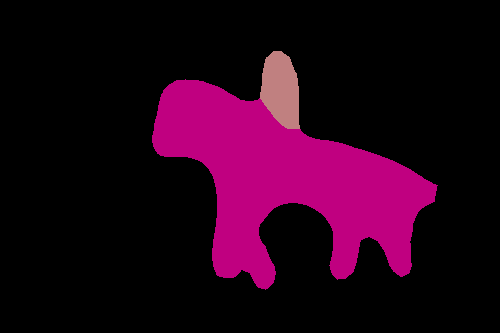
\includegraphics[height=0.11\linewidth]{fig/boundary_refine/vgg128noup_2007_003022.png} &
    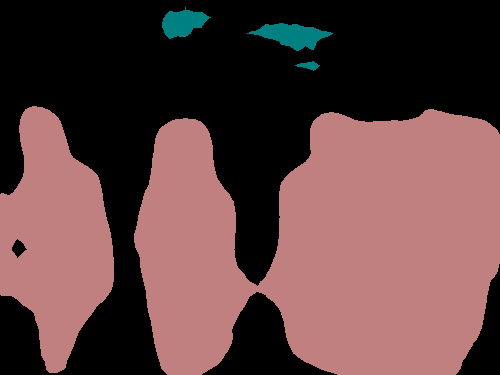
\includegraphics[height=0.11\linewidth]{fig/boundary_refine/vgg128noup_2007_001284.png} &
    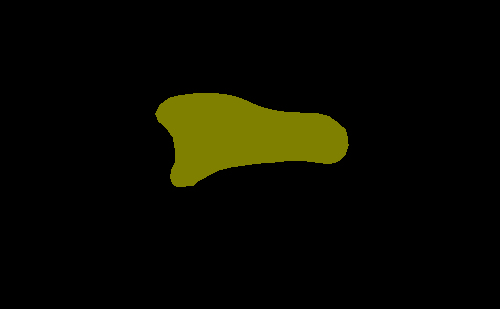
\includegraphics[height=0.11\linewidth]{fig/boundary_refine/vgg128noup_2007_001289.png} &
    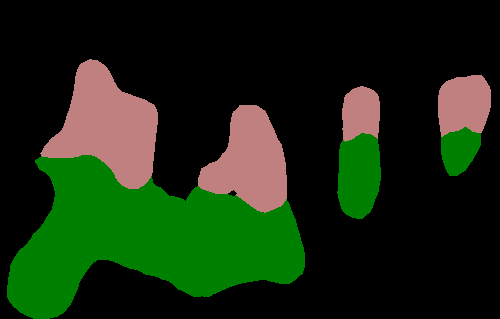
\includegraphics[height=0.11\linewidth]{fig/boundary_refine/vgg128noup_2007_001311.png} &
    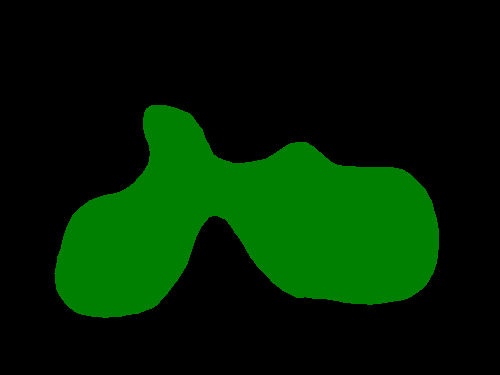
\includegraphics[height=0.11\linewidth]{fig/boundary_refine/vgg128noup_2009_000573.png} \\
    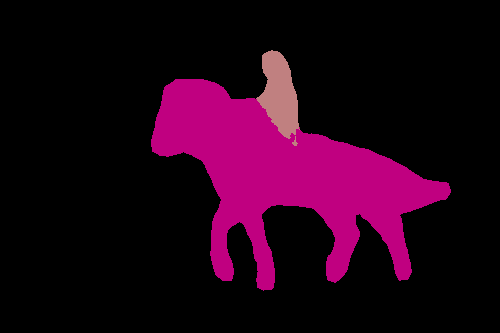
\includegraphics[height=0.11\linewidth]{fig/boundary_refine/vgg128ms_2007_003022.png} &
    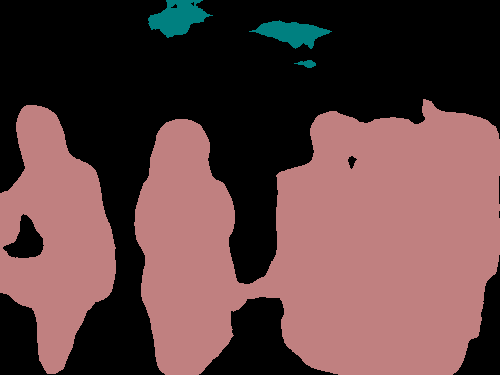
\includegraphics[height=0.11\linewidth]{fig/boundary_refine/vgg128ms_2007_001284.png} &
    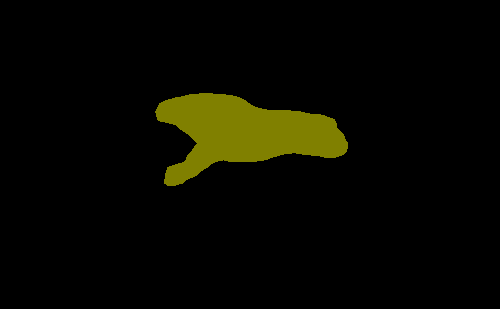
\includegraphics[height=0.11\linewidth]{fig/boundary_refine/vgg128ms_2007_001289.png} &
    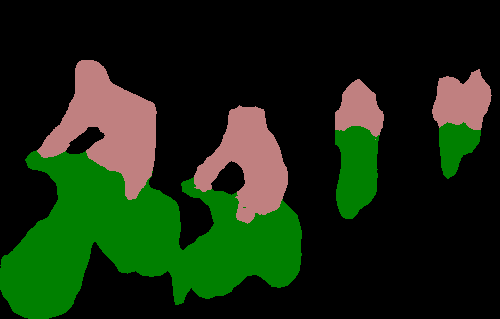
\includegraphics[height=0.11\linewidth]{fig/boundary_refine/vgg128ms_2007_001311.png} &
    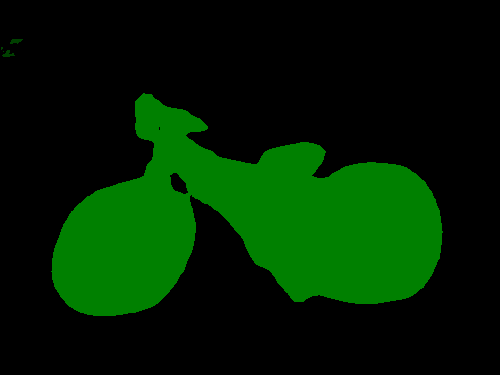
\includegraphics[height=0.11\linewidth]{fig/boundary_refine/vgg128ms_2009_000573.png} \\
  \end{tabular}
  \caption{Incorporating multi-scale features improves the boundary segmentation. We show the results obtained by DeepLab and DeepLab-MSc in the first and second row, respectively. Best viewed in color.}
  \label{fig:msBoundary}
\end{figure}

%{\bf{Weighted loss: }} In PASCAL VOC 2012 dataset, most of the pixels are labeled as background in the ground truths. Weighting the loss function according to the class frequency has been employed, \eg \citet{farabet2013learning, mostajabi2014feedforward}, to overcome the label imbalance problem. Our experiments on VOC 2012 val set show that using a weighted loss function increases the mean class accuracy (the pixelwise accuracy averaged across classes), but does not improve the mean IOU in our model. 

\paragraph{Mean Pixel IOU along Object Boundaries}
To quantify the accuracy of the proposed model near object boundaries, we evaluate the segmentation accuracy with an experiment similar to \citet{kohli2009robust, krahenbuhl2011efficient}. Specifically, we  use  the `void' label annotated in val set, which usually occurs around object boundaries. We compute the mean IOU for those pixels that are located within a narrow band (called trimap) of `void' labels. As shown in \figref{fig:IOUBoundary}, exploiting the multi-scale features from the intermediate layers and refining the segmentation results by a fully connected CRF significantly improve the results around object boundaries. 

\paragraph{Comparison with State-of-art} In \figref{fig:val_comparison}, we qualitatively compare our proposed model, DeepLab-CRF, with two state-of-art models: FCN-8s \citep{long2014fully} and TTI-Zoomout-16 \citep{mostajabi2014feedforward} on the `val' set (the results are extracted from their papers). Our model is able to capture the intricate object boundaries.

\begin{figure}[!tbp]
\centering
\resizebox{\columnwidth}{!}{
  \begin{tabular} {c c c}
%    \hspace{-0.5cm}\raisebox{2cm}
    \raisebox{1.7cm} {
    \begin{tabular}{c c}
      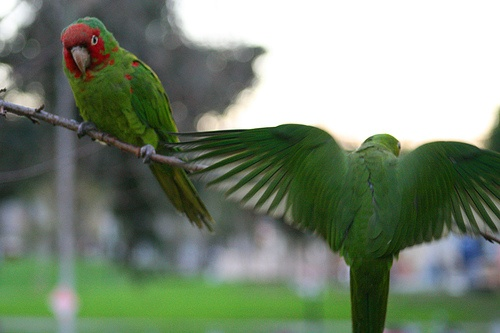
\includegraphics[height=0.1\linewidth]{fig/trimap/2007_000363.jpg} &
      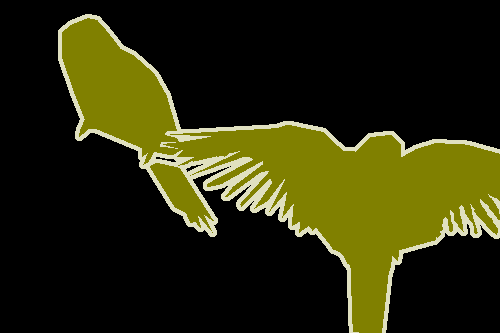
\includegraphics[height=0.1\linewidth]{fig/trimap/2007_000363.png} \\
      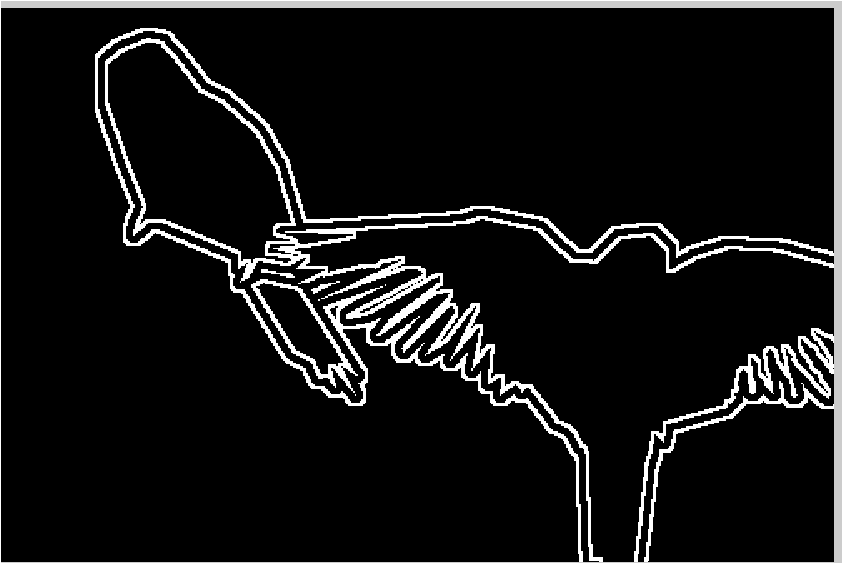
\includegraphics[height=0.1\linewidth]{fig/trimap/TrimapWidth2.pdf} &
      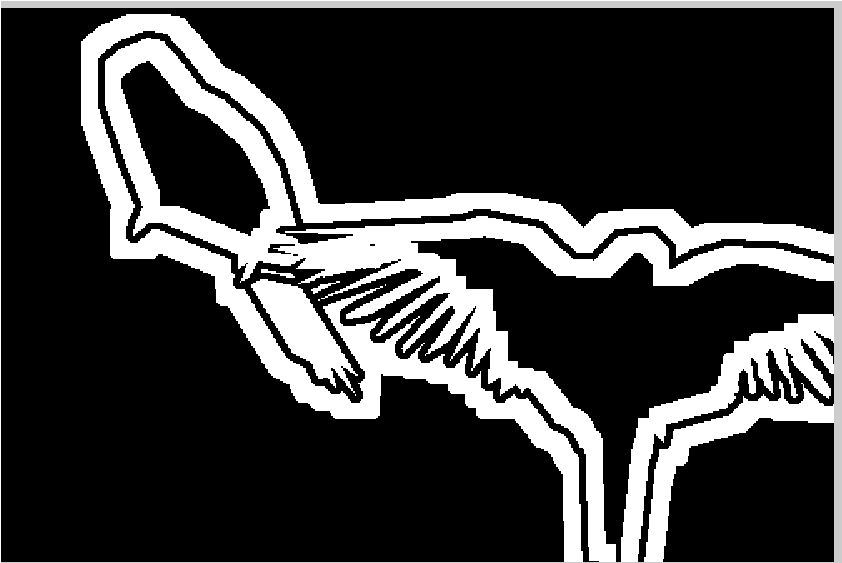
\includegraphics[height=0.1\linewidth]{fig/trimap/TrimapWidth10.pdf} \\
    \end{tabular} } &
    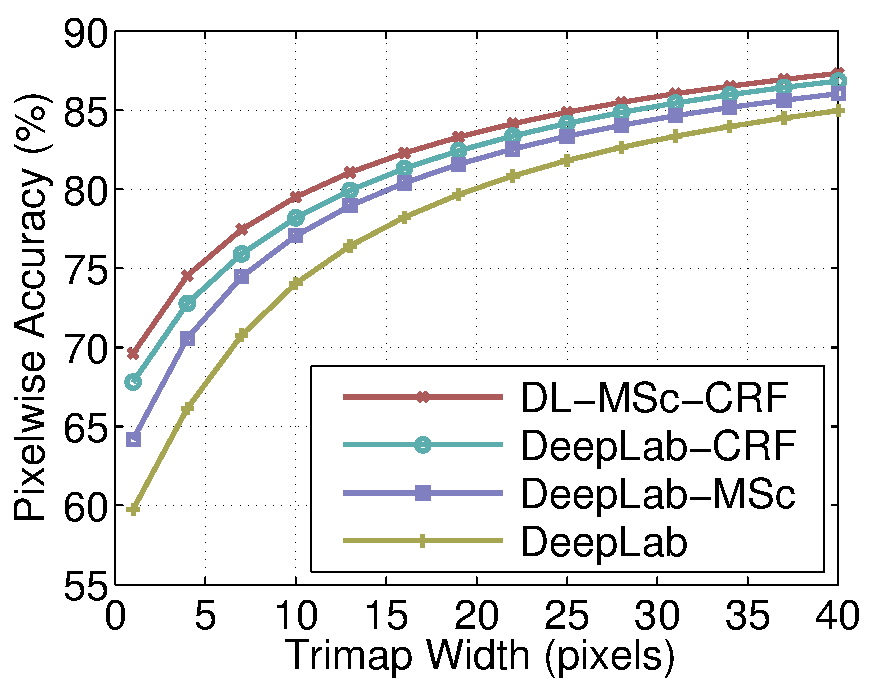
\includegraphics[height=0.25\linewidth]{fig/SegPixelAccWithinTrimap.pdf} &
    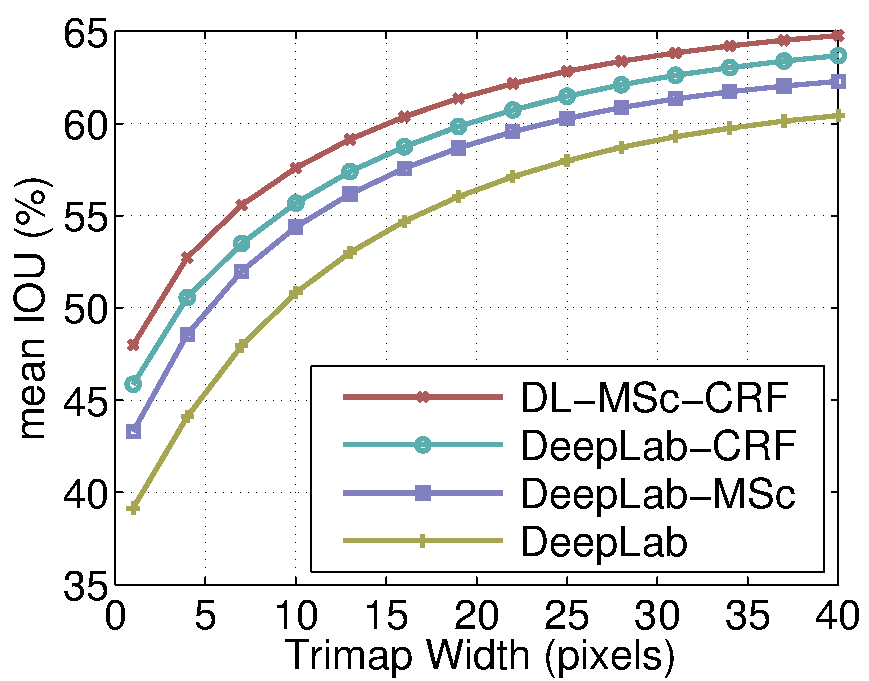
\includegraphics[height=0.25\linewidth]{fig/SegPixelIOUWithinTrimap.pdf} \\
    (a) & (b) & (c) \\
   \end{tabular}
}
  \caption{(a) Some trimap examples (top-left: image. top-right: ground-truth. bottom-left: trimap of 2 pixels. bottom-right: trimap of 10 pixels). Quality of segmentation result within a band around the object boundaries for the proposed methods. (b) Pixelwise accuracy. (c) Pixel mean IOU. 
    }  
  \label{fig:IOUBoundary}
\end{figure}


\begin{figure}[t]
  \centering
  \begin{tabular}{c c}
    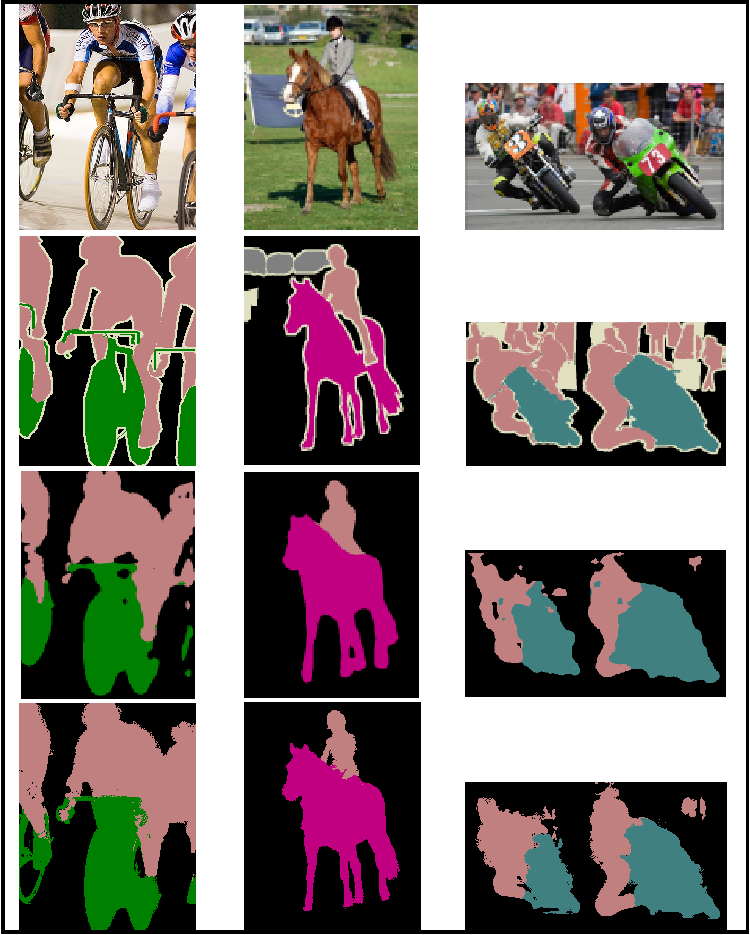
\includegraphics[height=0.55\linewidth]{fig/comparedWithFCN.pdf} &
    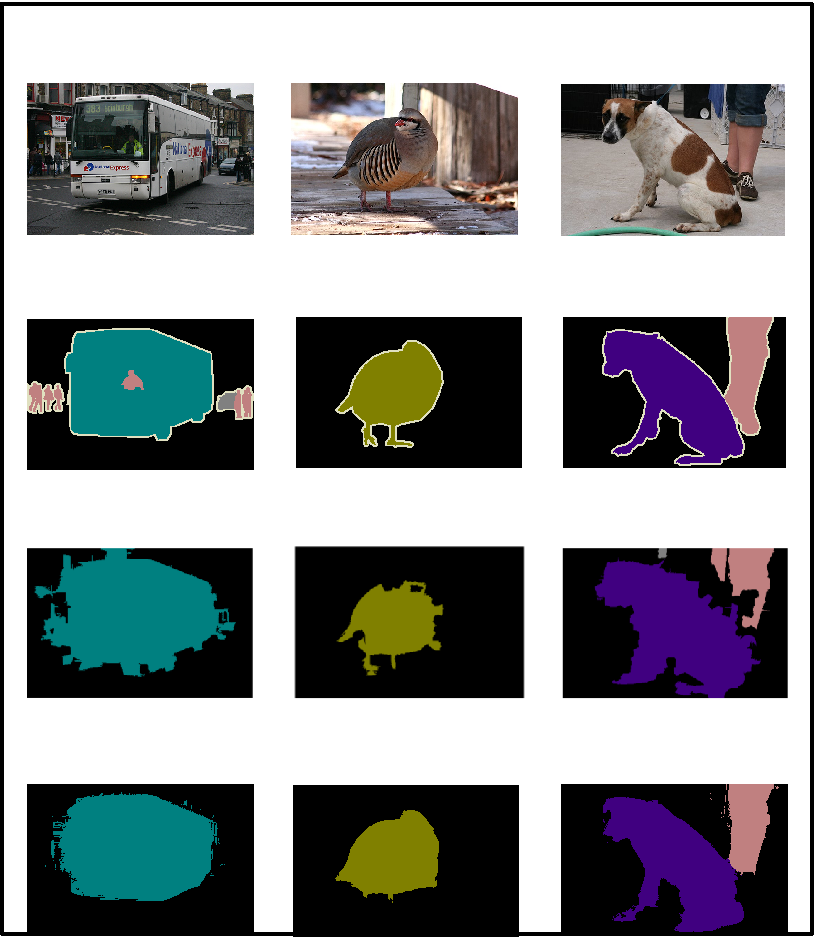
\includegraphics[height=0.55\linewidth]{fig/comparedWithRoomOut.pdf} \\
    (a) FCN-8s vs. DeepLab-CRF & (b) TTI-Zoomout-16 vs. DeepLab-CRF \\
  \end{tabular}
  \caption{Comparisons with state-of-the-art models on the val set. First row: images. Second row: ground truths. Third row: other recent models (Left: FCN-8s, Right: TTI-Zoomout-16). Fourth row: our DeepLab-CRF. Best viewed in color.}
  \label{fig:val_comparison}
\end{figure}


\paragraph{Test set results} Having set our model choices on the validation set, we evaluate our best model variant, DeepLab-CRF, on the PASCAL VOC 2012 official 'test' set.  As shown in \tabref{tab:voc2012}, our DeepLab-CRF and DeepLab-MSc-CRF models achieve performance of $66.4\%$ and $67.1\%$ mean IOU\footnote{\url{http://host.robots.ox.ac.uk:8080/leaderboard/displaylb.php?challengeid=11&compid=6}}, respectively. Our models outperform all the other state-of-the-art models (specifically, TTI-Zoomout-16 \citep{mostajabi2014feedforward}, FCN-8s \citep{long2014fully}, and MSRA-CFM \citep{dai2014convolutional}).

\begin{table*}[!tbp]\scriptsize
\setlength{\tabcolsep}{3pt}
%\hspace{-1.8cm}
\resizebox{\columnwidth}{!}{
\begin{tabular}{|c||c*{20}{|c}||c|}
\hline 
Method         & bkg &  aero & bike & bird & boat & bottle& bus & car  &  cat & chair& cow  &table & dog  & horse & mbike& person& plant&sheep& sofa &train & tv   & mean \\
\hline \hline
MSRA-CFM       & -    & 75.7 & 26.7 & 69.5 & 48.8 & 65.6 & 81.0 & 69.2 & 73.3 & {\bf 30.0} & 68.7 & 51.5 & 69.1 & 68.1  & 71.7 & 67.5 & 50.4 & 66.5 & 44.4 & 58.9 & 53.5 & 61.8 \\
FCN-8s         & -    & 76.8 & 34.2 & 68.9 & 49.4 & 60.3 & 75.3 & 74.7 & 77.6 & 21.4 & 62.5 & 46.8 & 71.8 & 63.9  & 76.5 & 73.9 & 45.2 & 72.4 & 37.4 & 70.9 & 55.1 & 62.2 \\
TTI-Zoomout-16 & 89.8 & {\bf 81.9} & 35.1 & {\bf 78.2} & {\bf 57.4} & 56.5 & 80.5 & 74.0 & {\bf 79.8} & 22.4 & {\bf 69.6} & {\bf 53.7} & 74.0 & {\bf 76.0} & 76.6 & 68.8 & 44.3 & 70.2 & 40.2 & 68.9 & 55.3 & 64.4 \\
\hline
DeepLab-CRF    & 92.1 & 78.4 & 33.1 & {\bf 78.2} & 55.6 & 65.3 & 81.3 & 75.5 & 78.6 & 25.3 & 69.2 & 52.7 & {\bf 75.2} & 69.0  & 79.1 & 77.6 & 54.7 & 78.3 & 45.1 & {\bf 73.3} & 56.2 & 66.4 \\ 
DeepLab-MSc-CRF & {\bf 92.6} & 80.4 & {\bf 36.8} & 77.4 & 55.2 & {\bf 66.4} & {\bf 81.5} & {\bf 77.5} & 78.9 & 27.1 & 68.2 & 52.7 & 74.3 & 69.6 & {\bf 79.4} & {\bf 79.0} & {\bf 56.9} & {\bf 78.8} & {\bf 45.2} & 72.7 & {\bf 59.3} & {\bf 67.1} \\
\hline
 \end{tabular}
}
 \caption{Labeling IOU (\%) on the PASCAL VOC 2012 test set, using the trainval set for training.}
 \label{tab:voc2012}
\end{table*}



% \begin{figure}[ht]
%   \centering
%   \begin{tabular}{c c c | c c}
%     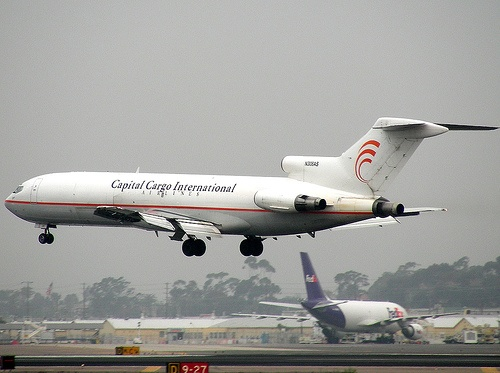
\includegraphics[height=0.12\linewidth]{fig/img/2007_002266.jpg} &
%     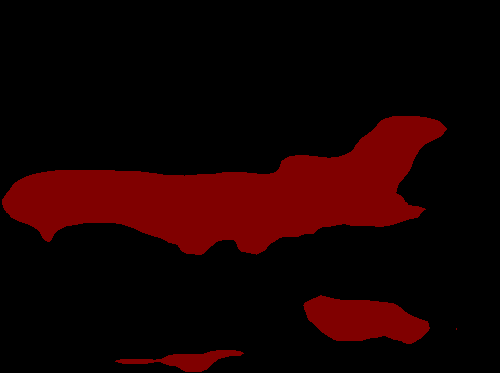
\includegraphics[height=0.12\linewidth]{fig/fcn8s/2007_002266.png} &
%     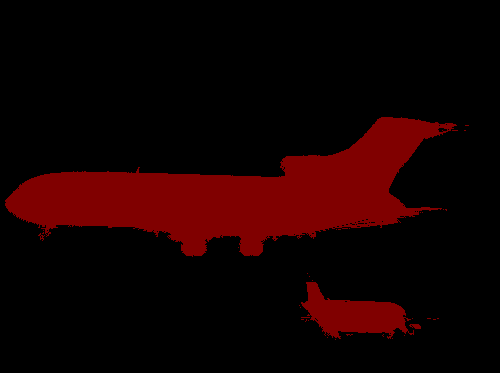
\includegraphics[height=0.12\linewidth]{fig/res_crf/2007_002266.png} &
%     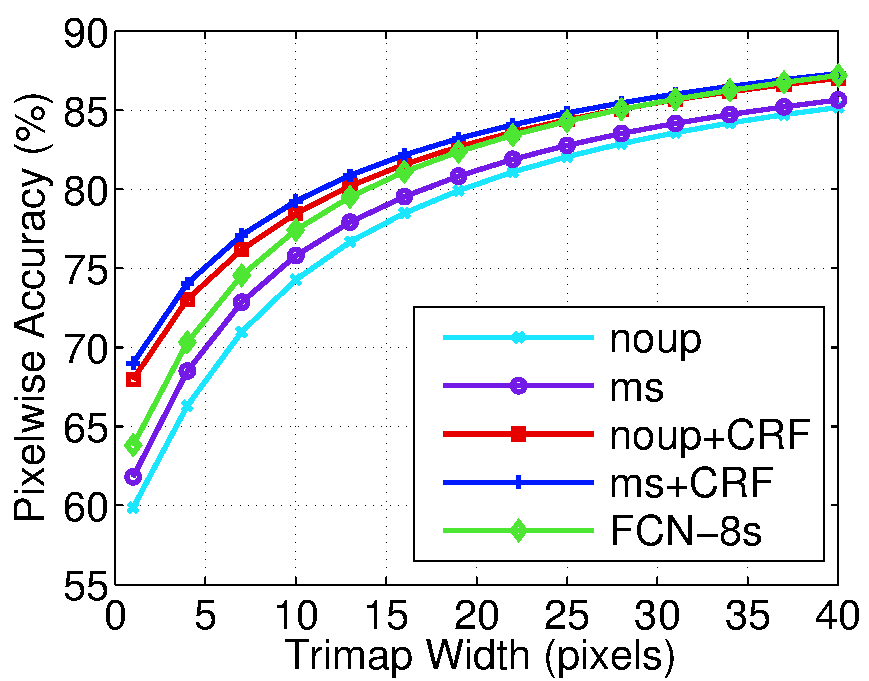
\includegraphics[height=0.12\linewidth]{fig/SegPixelAccWithinTrimap_Berkeley.pdf} &
%     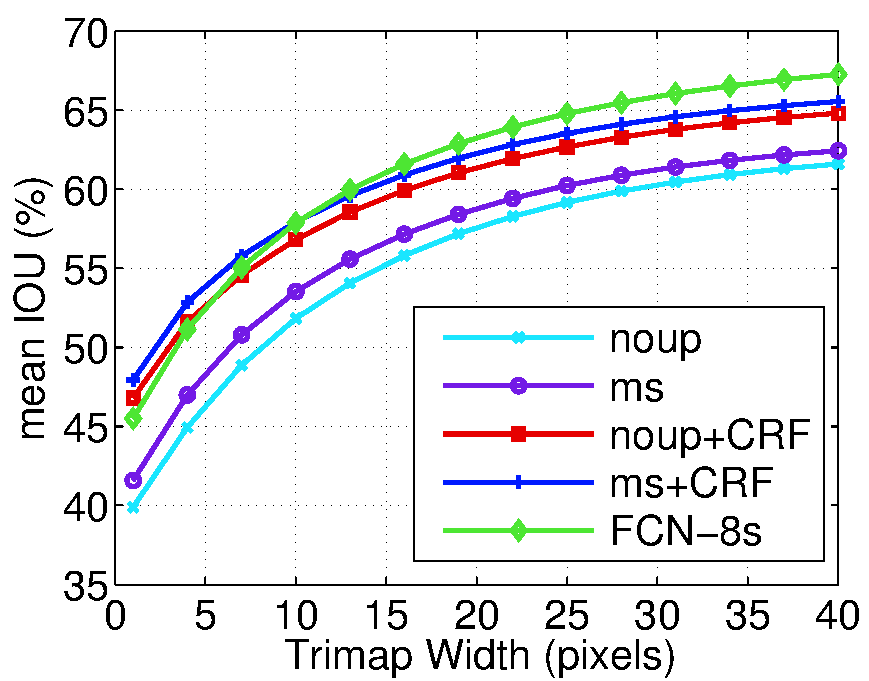
\includegraphics[height=0.12\linewidth]{fig/SegPixelIOUWithinTrimap_Berkeley.pdf} \\
%     (a) & (b) & (c) & (d) & (e)
%   \end{tabular}
%   \caption{(Left) Some comparisons with FCN-8S: (a) image; (b) FCN-8S; (c)
%     ms-crf. (d) Segmentation accuracy (pixelwise accuracy) within trimap. (e)
%     Segmentation accuracy (mean IOU) within trimap. {\color{red} TODO: change
%       legend. HELP: I cannot make them equally spaced....}} 
%   \label{fig:IOUBoundary}
% \end{figure}

\begin{figure}[!htbp]
  \centering
  %\vspace{-1.cm}
  \scalebox{0.82} {
  \begin{tabular}{c c c | c c c}
    %\addtolength{\tabcolsep}{-6.5pt}
    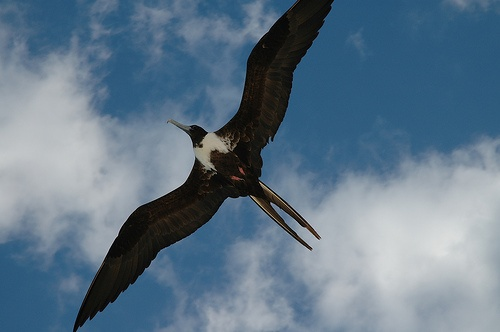
\includegraphics[height=0.12\linewidth]{fig/img/2007_002094.jpg} &
    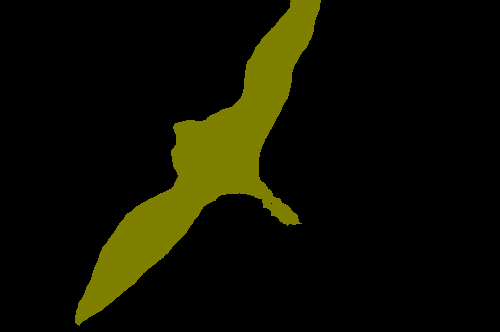
\includegraphics[height=0.12\linewidth]{fig/res_none/2007_002094.png} &
    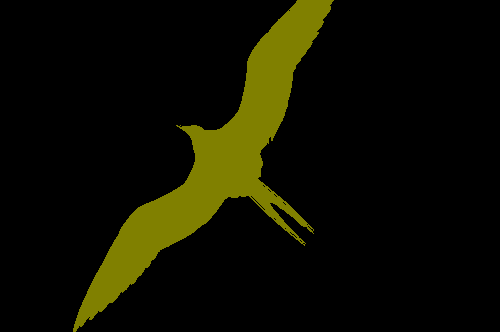
\includegraphics[height=0.12\linewidth]{fig/res_crf/2007_002094.png} &
    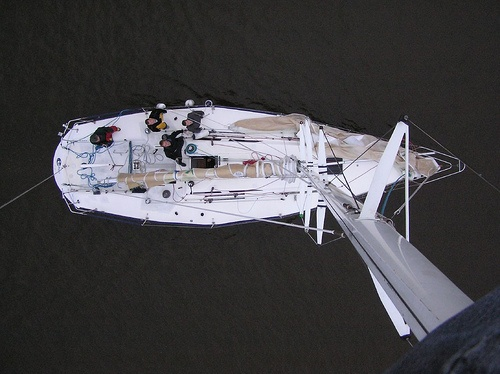
\includegraphics[height=0.12\linewidth]{fig/img/2007_002719.jpg} &
    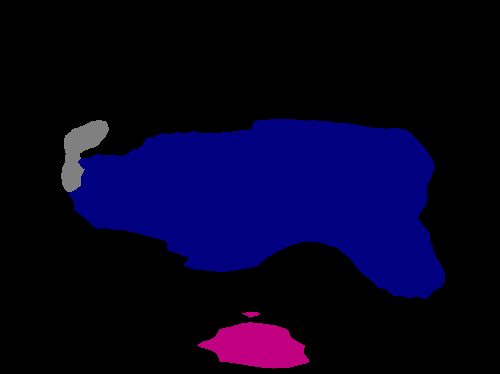
\includegraphics[height=0.12\linewidth]{fig/res_none/2007_002719.png} &
    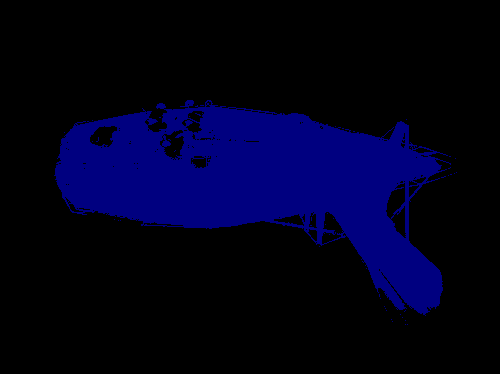
\includegraphics[height=0.12\linewidth]{fig/res_crf/2007_002719.png} \\
    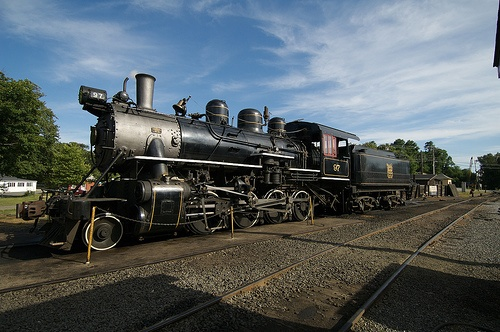
\includegraphics[height=0.12\linewidth]{fig/img/2007_003957.jpg} &
    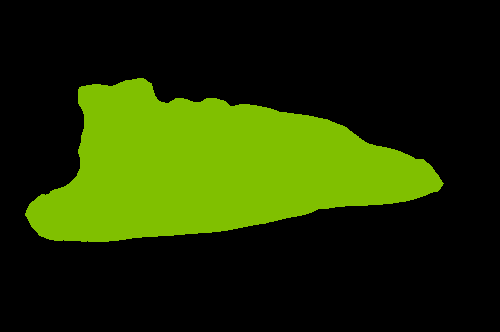
\includegraphics[height=0.12\linewidth]{fig/res_none/2007_003957.png} &
    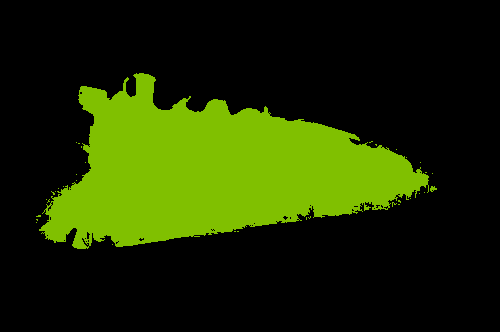
\includegraphics[height=0.12\linewidth]{fig/res_crf/2007_003957.png} &
    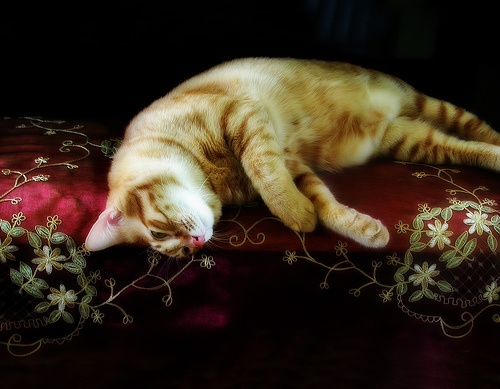
\includegraphics[height=0.12\linewidth]{fig/img/2007_003991.jpg} &
    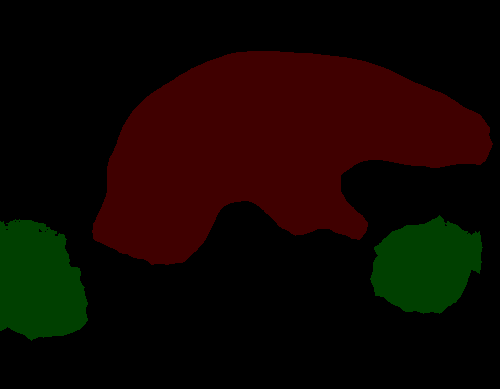
\includegraphics[height=0.12\linewidth]{fig/res_none/2007_003991.png} &
    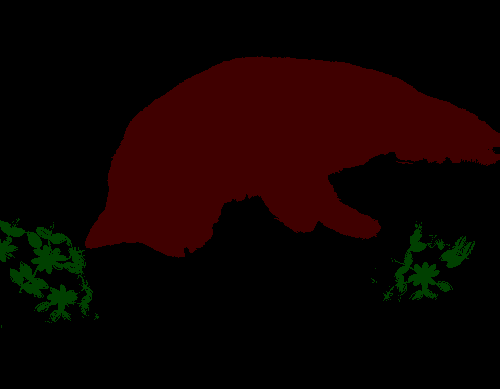
\includegraphics[height=0.12\linewidth]{fig/res_crf/2007_003991.png} \\
    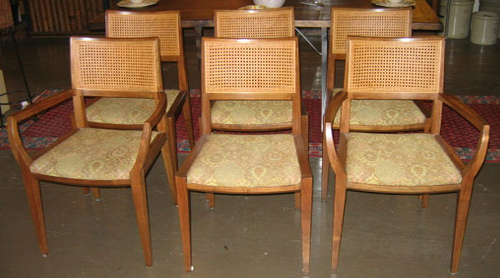
\includegraphics[height=0.10\linewidth]{fig/img/2008_001439.jpg} &
    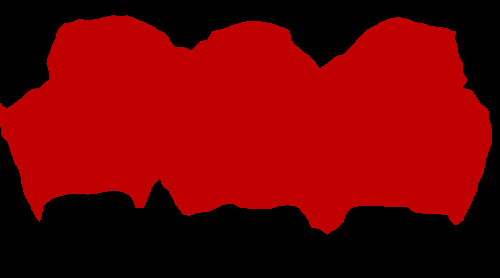
\includegraphics[height=0.10\linewidth]{fig/res_none/2008_001439.png} &
    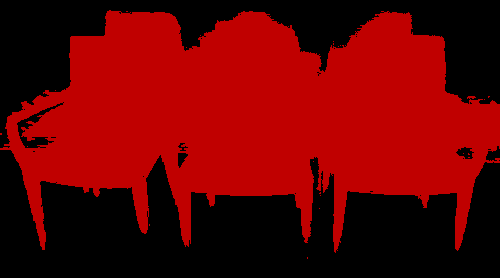
\includegraphics[height=0.10\linewidth]{fig/res_crf/2008_001439.png} &
    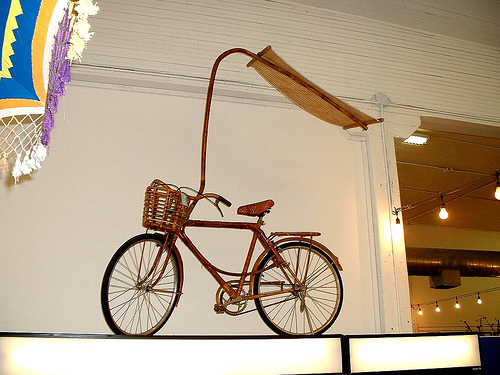
\includegraphics[height=0.12\linewidth]{fig/img/2008_004363.jpg} &
    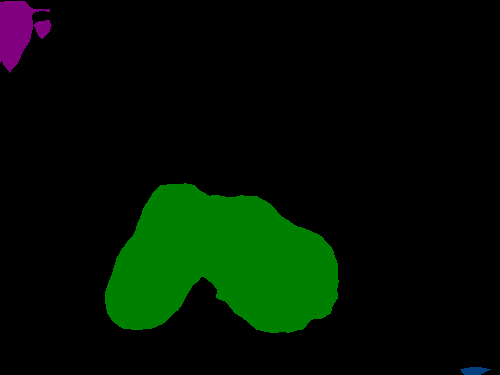
\includegraphics[height=0.12\linewidth]{fig/res_none/2008_004363.png} &
    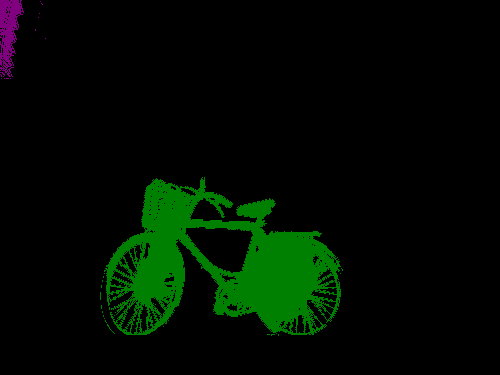
\includegraphics[height=0.12\linewidth]{fig/res_crf/2008_004363.png} \\
    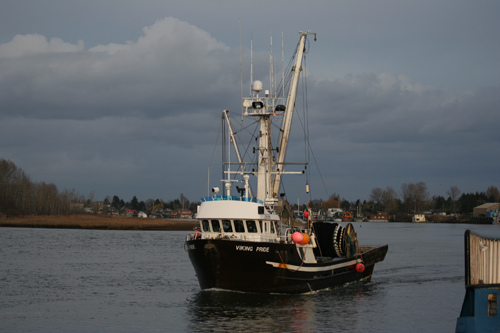
\includegraphics[height=0.12\linewidth]{fig/img/2008_006229.jpg} &
    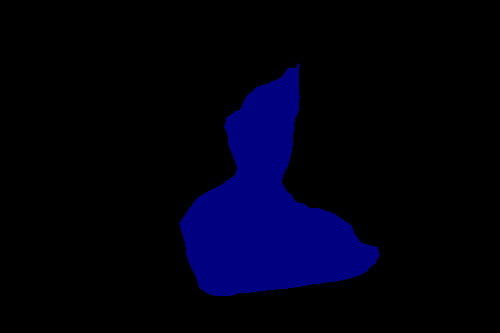
\includegraphics[height=0.12\linewidth]{fig/res_none/2008_006229.png} &
    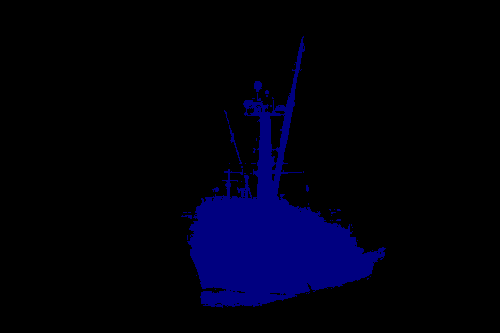
\includegraphics[height=0.12\linewidth]{fig/res_crf/2008_006229.png} &
    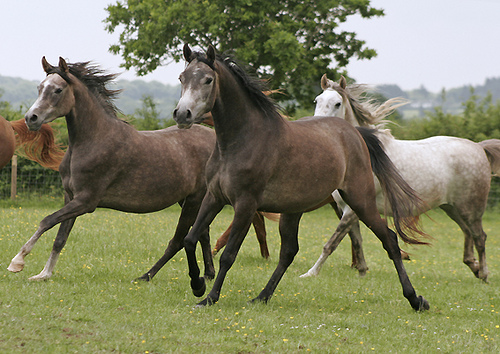
\includegraphics[height=0.12\linewidth]{fig/img/2009_000412.jpg} &
    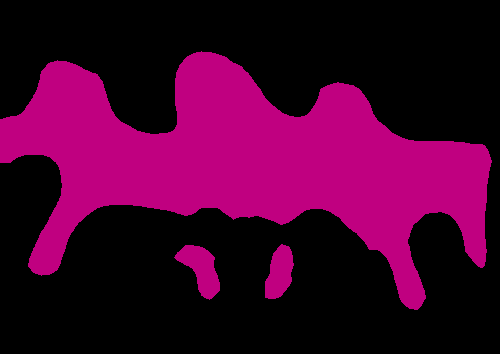
\includegraphics[height=0.12\linewidth]{fig/res_none/2009_000412.png} &
    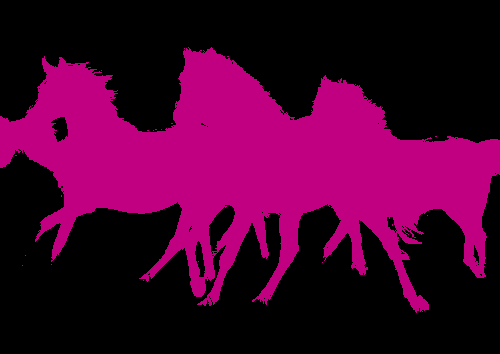
\includegraphics[height=0.12\linewidth]{fig/res_crf/2009_000412.png} \\
    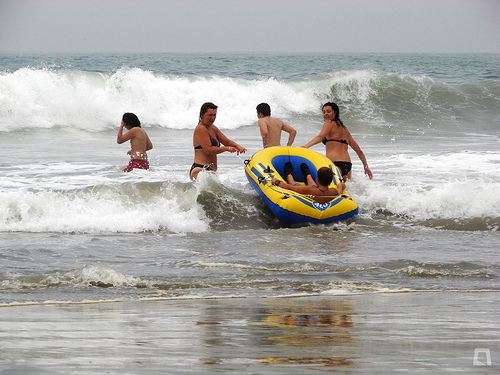
\includegraphics[height=0.12\linewidth]{fig/img/2009_000421.jpg} &
    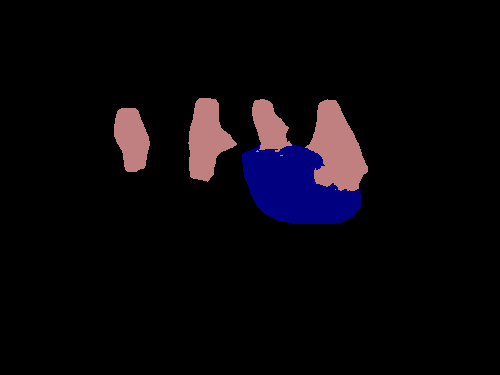
\includegraphics[height=0.12\linewidth]{fig/res_none/2009_000421.png} &
    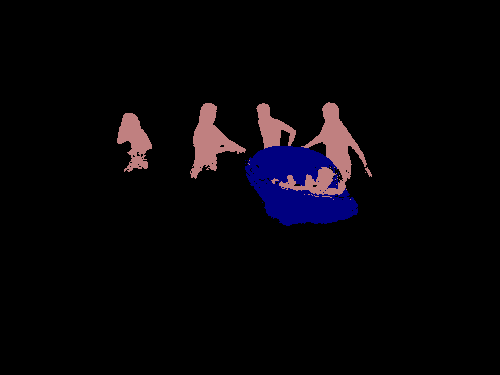
\includegraphics[height=0.12\linewidth]{fig/res_crf/2009_000421.png} &
    \includegraphics[height=0.12\linewidth]{fig/img/2010_001079.jpg} &
    \includegraphics[height=0.12\linewidth]{fig/res_none/2010_001079.png} &
    \includegraphics[height=0.12\linewidth]{fig/res_crf/2010_001079.png} \\
    \includegraphics[height=0.12\linewidth]{fig/img/2010_000038.jpg} &
    \includegraphics[height=0.12\linewidth]{fig/res_none/2010_000038.png} &
    \includegraphics[height=0.12\linewidth]{fig/res_crf/2010_000038.png} &
    \includegraphics[height=0.12\linewidth]{fig/img/2010_001024.jpg} &
    \includegraphics[height=0.12\linewidth]{fig/res_none/2010_001024.png} &
    \includegraphics[height=0.12\linewidth]{fig/res_crf/2010_001024.png} \\
    \includegraphics[height=0.24\linewidth]{fig/img/2007_005331.jpg} &
    \includegraphics[height=0.24\linewidth]{fig/res_none/2007_005331.png} &
    \includegraphics[height=0.24\linewidth]{fig/res_crf/2007_005331.png} &
    \includegraphics[height=0.24\linewidth]{fig/img/2008_004654.jpg} &
    \includegraphics[height=0.24\linewidth]{fig/res_none/2008_004654.png} &
    \includegraphics[height=0.24\linewidth]{fig/res_crf/2008_004654.png} \\
    \includegraphics[height=0.24\linewidth]{fig/img/2007_000129.jpg} &
    \includegraphics[height=0.24\linewidth]{fig/res_none/2007_000129.png} &
    \includegraphics[height=0.24\linewidth]{fig/res_crf/2007_000129.png} &
    \includegraphics[height=0.24\linewidth]{fig/img/2007_002619.jpg} &
    \includegraphics[height=0.24\linewidth]{fig/res_none/2007_002619.png} &
    \includegraphics[height=0.24\linewidth]{fig/res_crf/2007_002619.png} \\
    \includegraphics[height=0.12\linewidth]{fig/img/2007_002852.jpg} &
    \includegraphics[height=0.12\linewidth]{fig/res_none/2007_002852.png} &
    \includegraphics[height=0.12\linewidth]{fig/res_crf/2007_002852.png} &
    \includegraphics[height=0.12\linewidth]{fig/img/2010_001069.jpg} &
    \includegraphics[height=0.12\linewidth]{fig/res_none/2010_001069.png} &
    \includegraphics[height=0.12\linewidth]{fig/res_crf/2010_001069.png} \\
    \hline
    \hline
    \includegraphics[height=0.12\linewidth]{fig/img/2007_000491.jpg} &
    \includegraphics[height=0.12\linewidth]{fig/res_none/2007_000491.png} &
    \includegraphics[height=0.12\linewidth]{fig/res_crf/2007_000491.png} &
    \includegraphics[height=0.12\linewidth]{fig/img/2007_000529.jpg} &
    \includegraphics[height=0.12\linewidth]{fig/res_none/2007_000529.png} &
    \includegraphics[height=0.12\linewidth]{fig/res_crf/2007_000529.png} \\
    \includegraphics[height=0.12\linewidth]{fig/img/2007_000559.jpg} &
    \includegraphics[height=0.12\linewidth]{fig/res_none/2007_000559.png} &
    \includegraphics[height=0.12\linewidth]{fig/res_crf/2007_000559.png} &
    \includegraphics[height=0.12\linewidth]{fig/img/2007_000663.jpg} &
    \includegraphics[height=0.12\linewidth]{fig/res_none/2007_000663.png} &
    \includegraphics[height=0.12\linewidth]{fig/res_crf/2007_000663.png} \\    
    \includegraphics[height=0.12\linewidth]{fig/img/2007_000452.jpg} &
    \includegraphics[height=0.12\linewidth]{fig/res_none/2007_000452.png} &
    \includegraphics[height=0.12\linewidth]{fig/res_crf/2007_000452.png} &
    \includegraphics[height=0.12\linewidth]{fig/img/2007_002268.jpg} &
    \includegraphics[height=0.12\linewidth]{fig/res_none/2007_002268.png} &
    \includegraphics[height=0.12\linewidth]{fig/res_crf/2007_002268.png} \\
  \end{tabular}
  }
  %\vspace{-0.3cm}
  \caption{Visualization results on VOC 2012-val. For each row, we show the input image, the segmentation result delivered by the DCNN (DeepLab), and the refined segmentation result of the Fully Connected CRF (DeepLab-CRF). We show our failure modes in the last three rows. Best viewed in color.} 
  \label{fig:ValResults}
\end{figure}
